\documentclass[main.tex]{subfiles}
\begin{document}
{\Huge {ಒಂದು ಎರಡು}
\large
\begin{poem}
  \raggedleft
  \begin{stanza}
    ಒಂದು ಎರಡು ಬಾಳೆಲೆ ಹರಡು \verseline
    \AddToShipoutPicture*{
      \put(-10,30){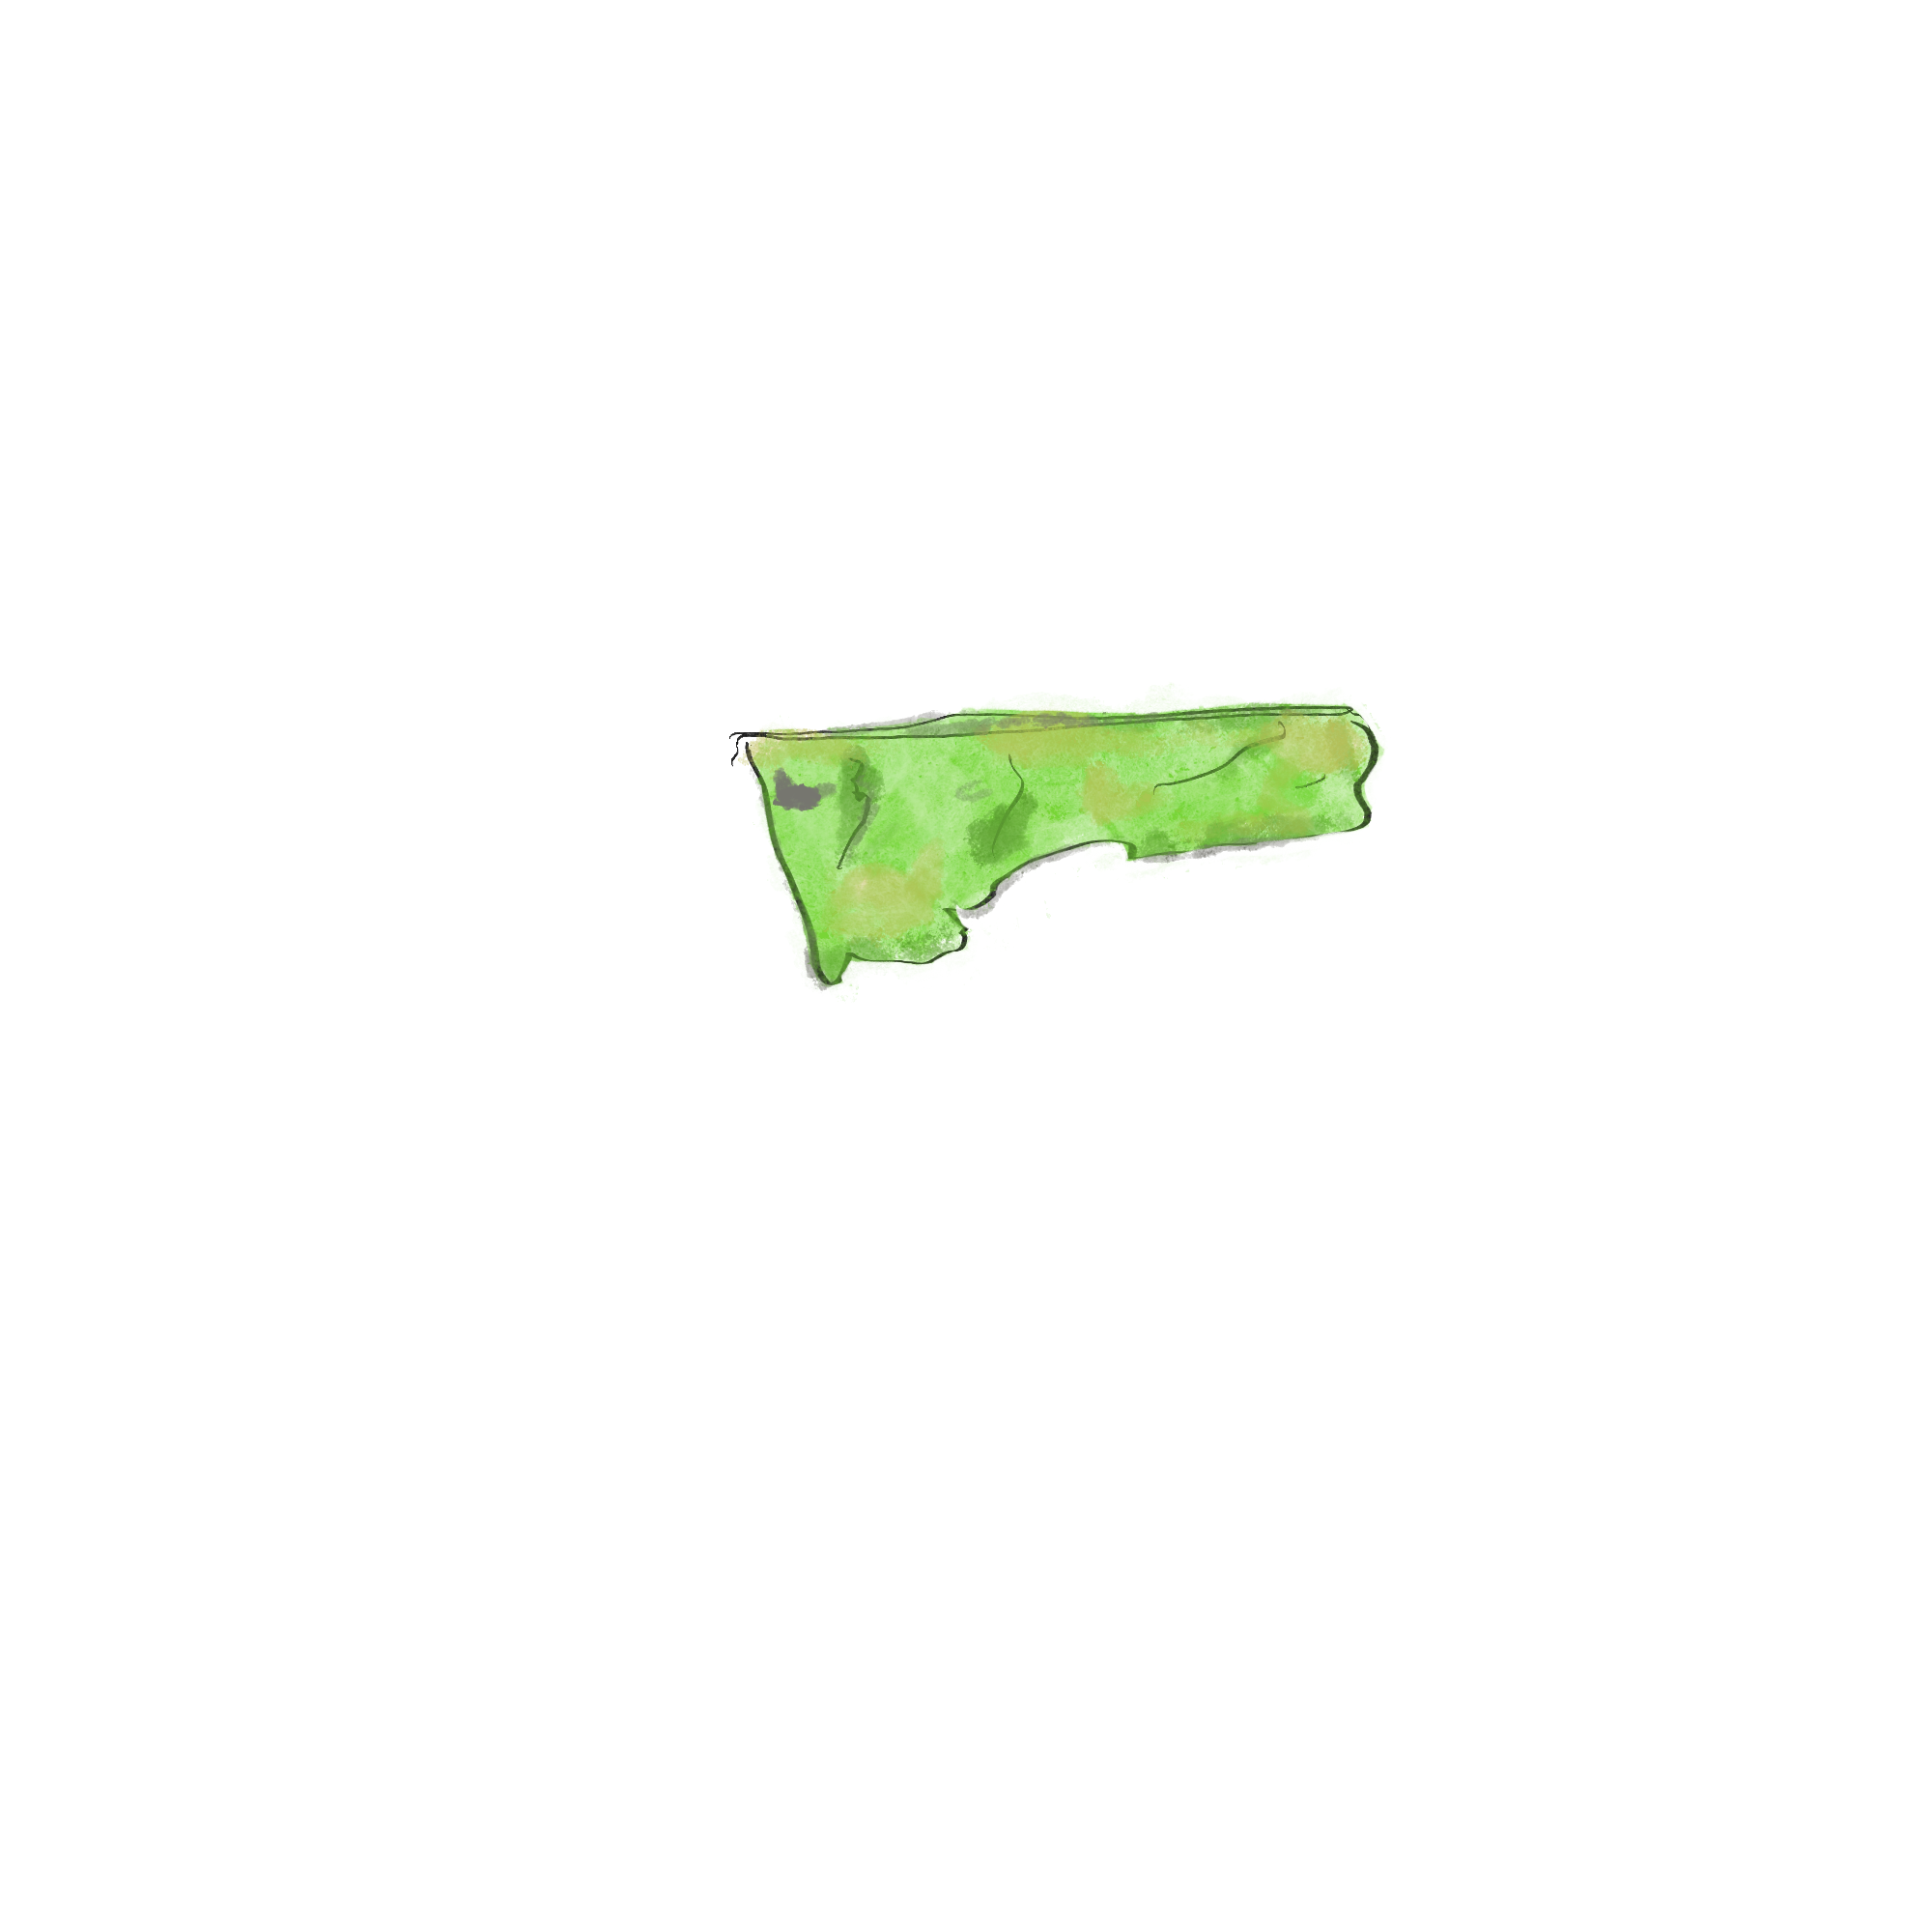
\includegraphics[width=5.0cm]{ele5.png}} % Adjust the coordinates and size as needed
    }
    \AddToShipoutPicture*{
      \put(30,130){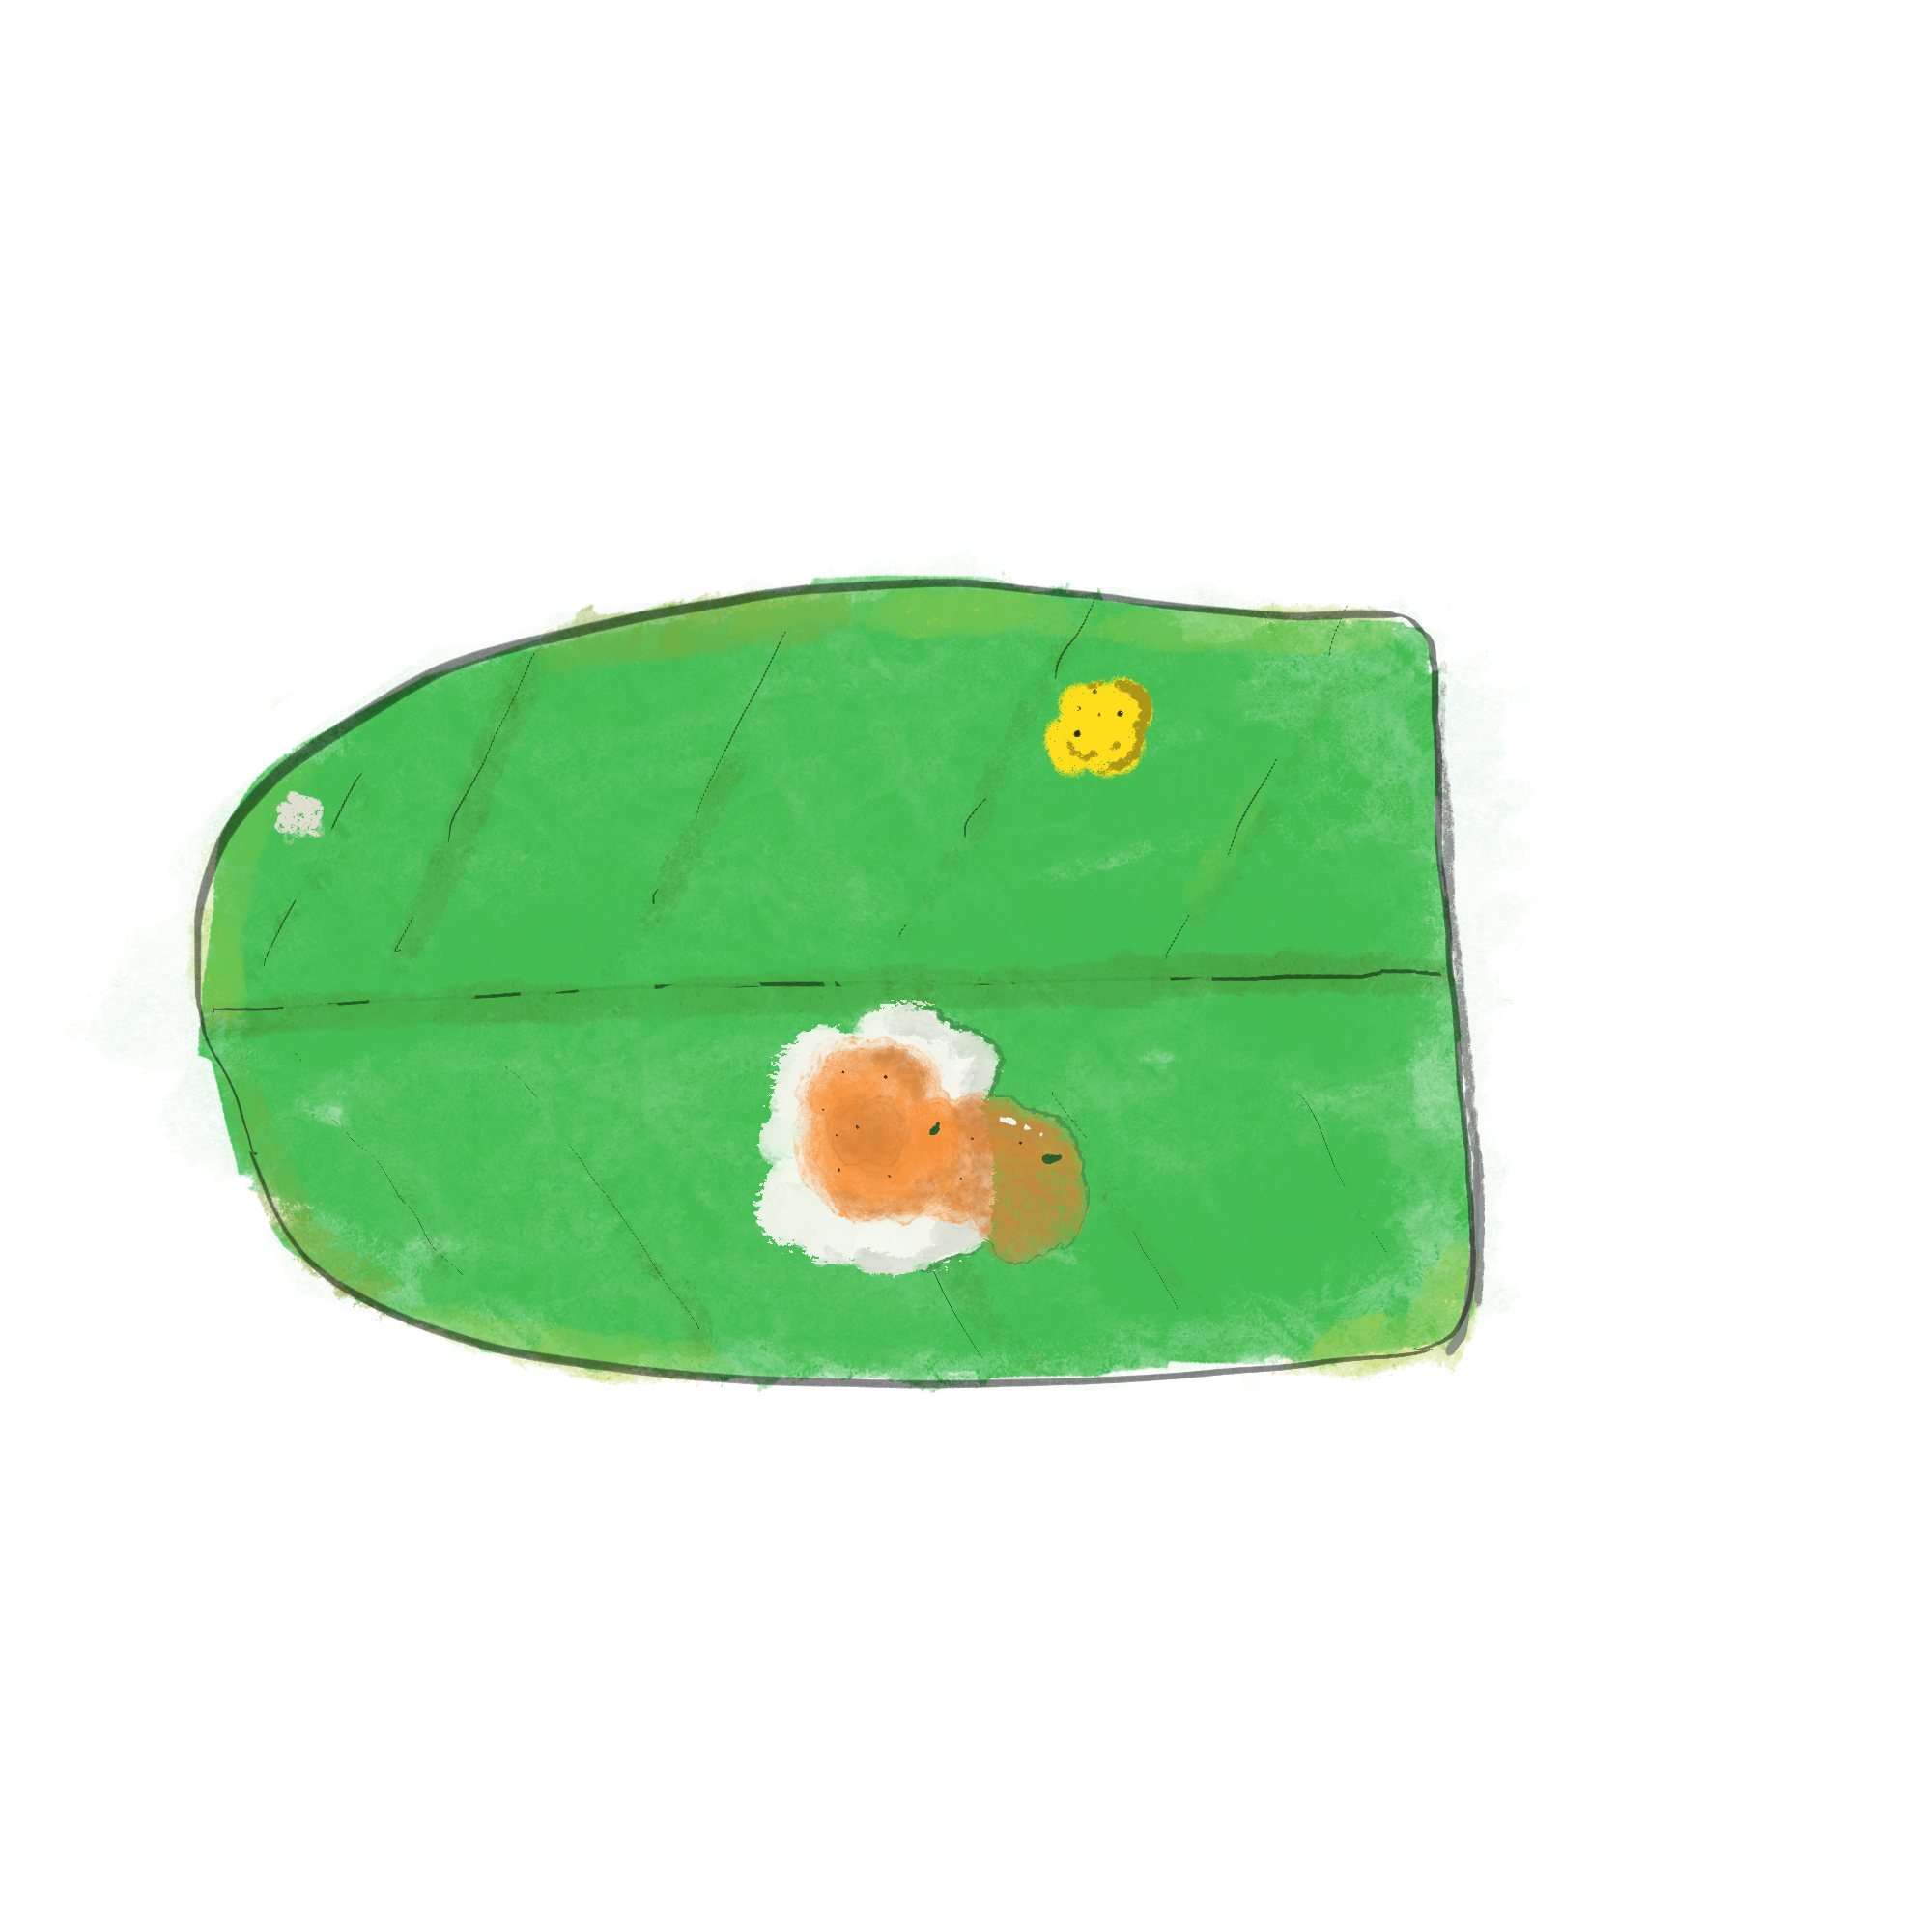
\includegraphics[width=4.0cm]{ele4.png}} % Adjust the coordinates and size as needed
    }
    \AddToShipoutPicture*{
      \put(30,230){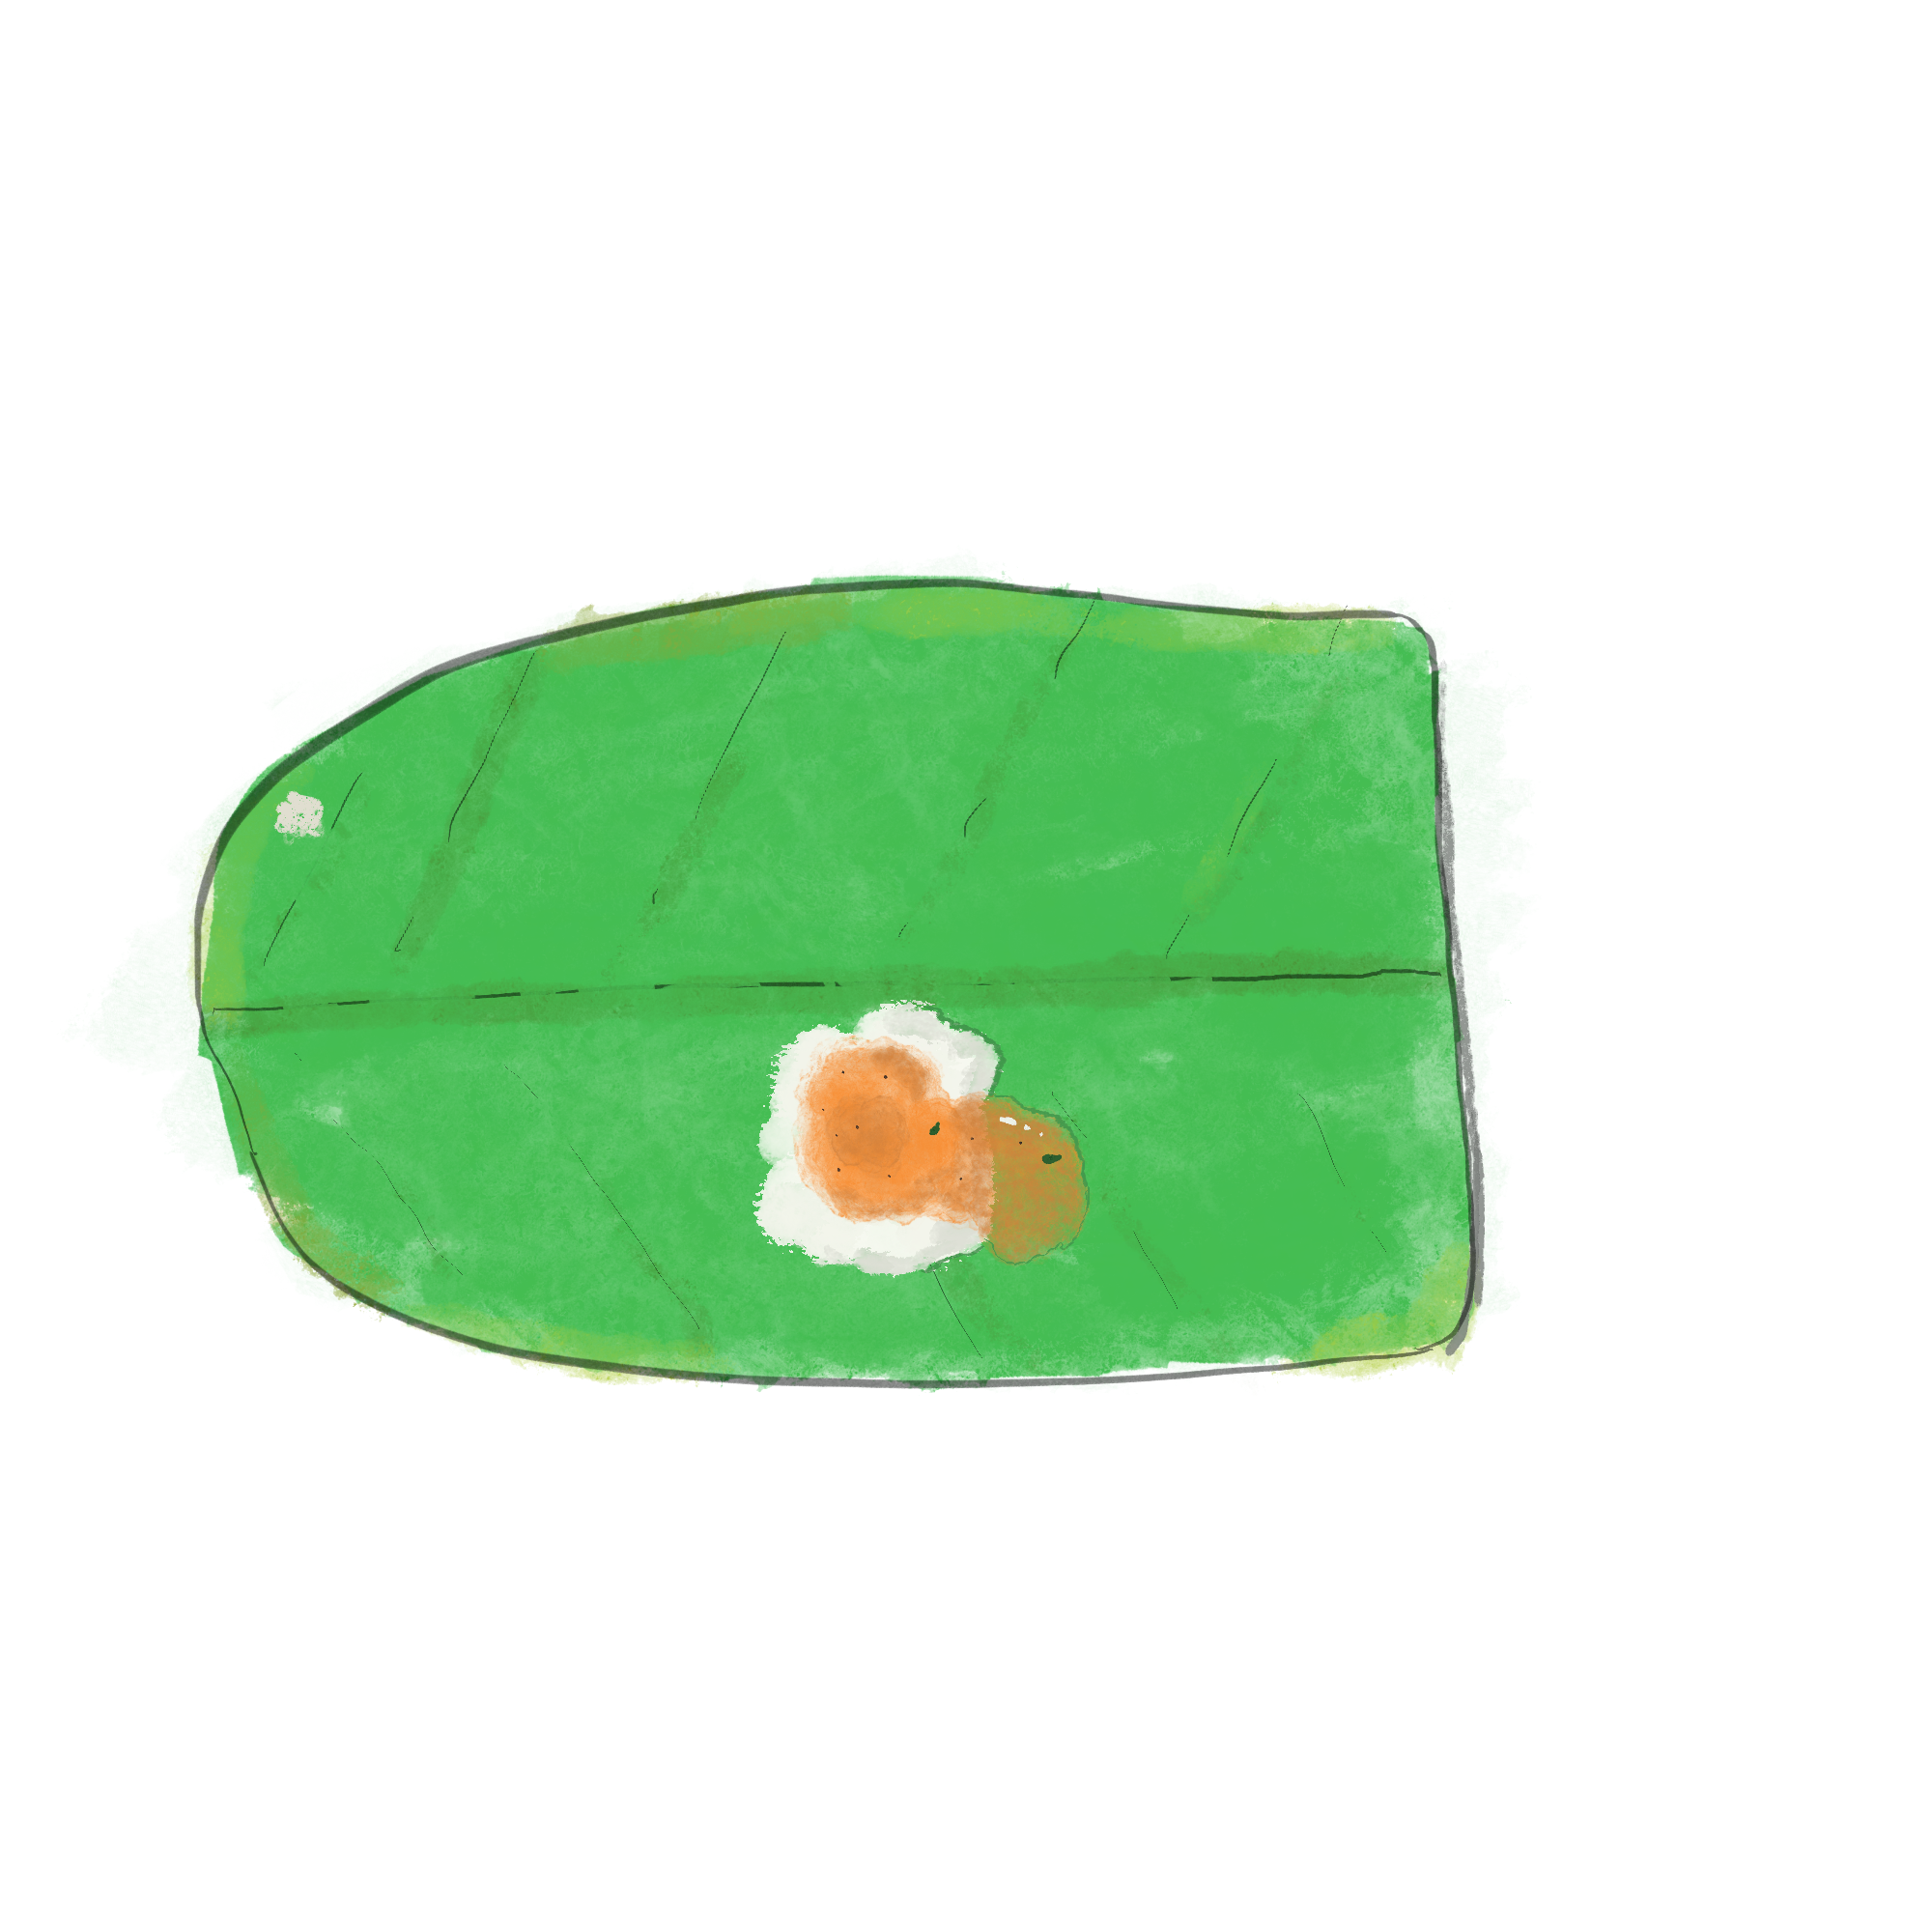
\includegraphics[width=4.0cm]{ele3.png}} % Adjust the coordinates and size as needed
    }
    \AddToShipoutPicture*{
      \put(30,330){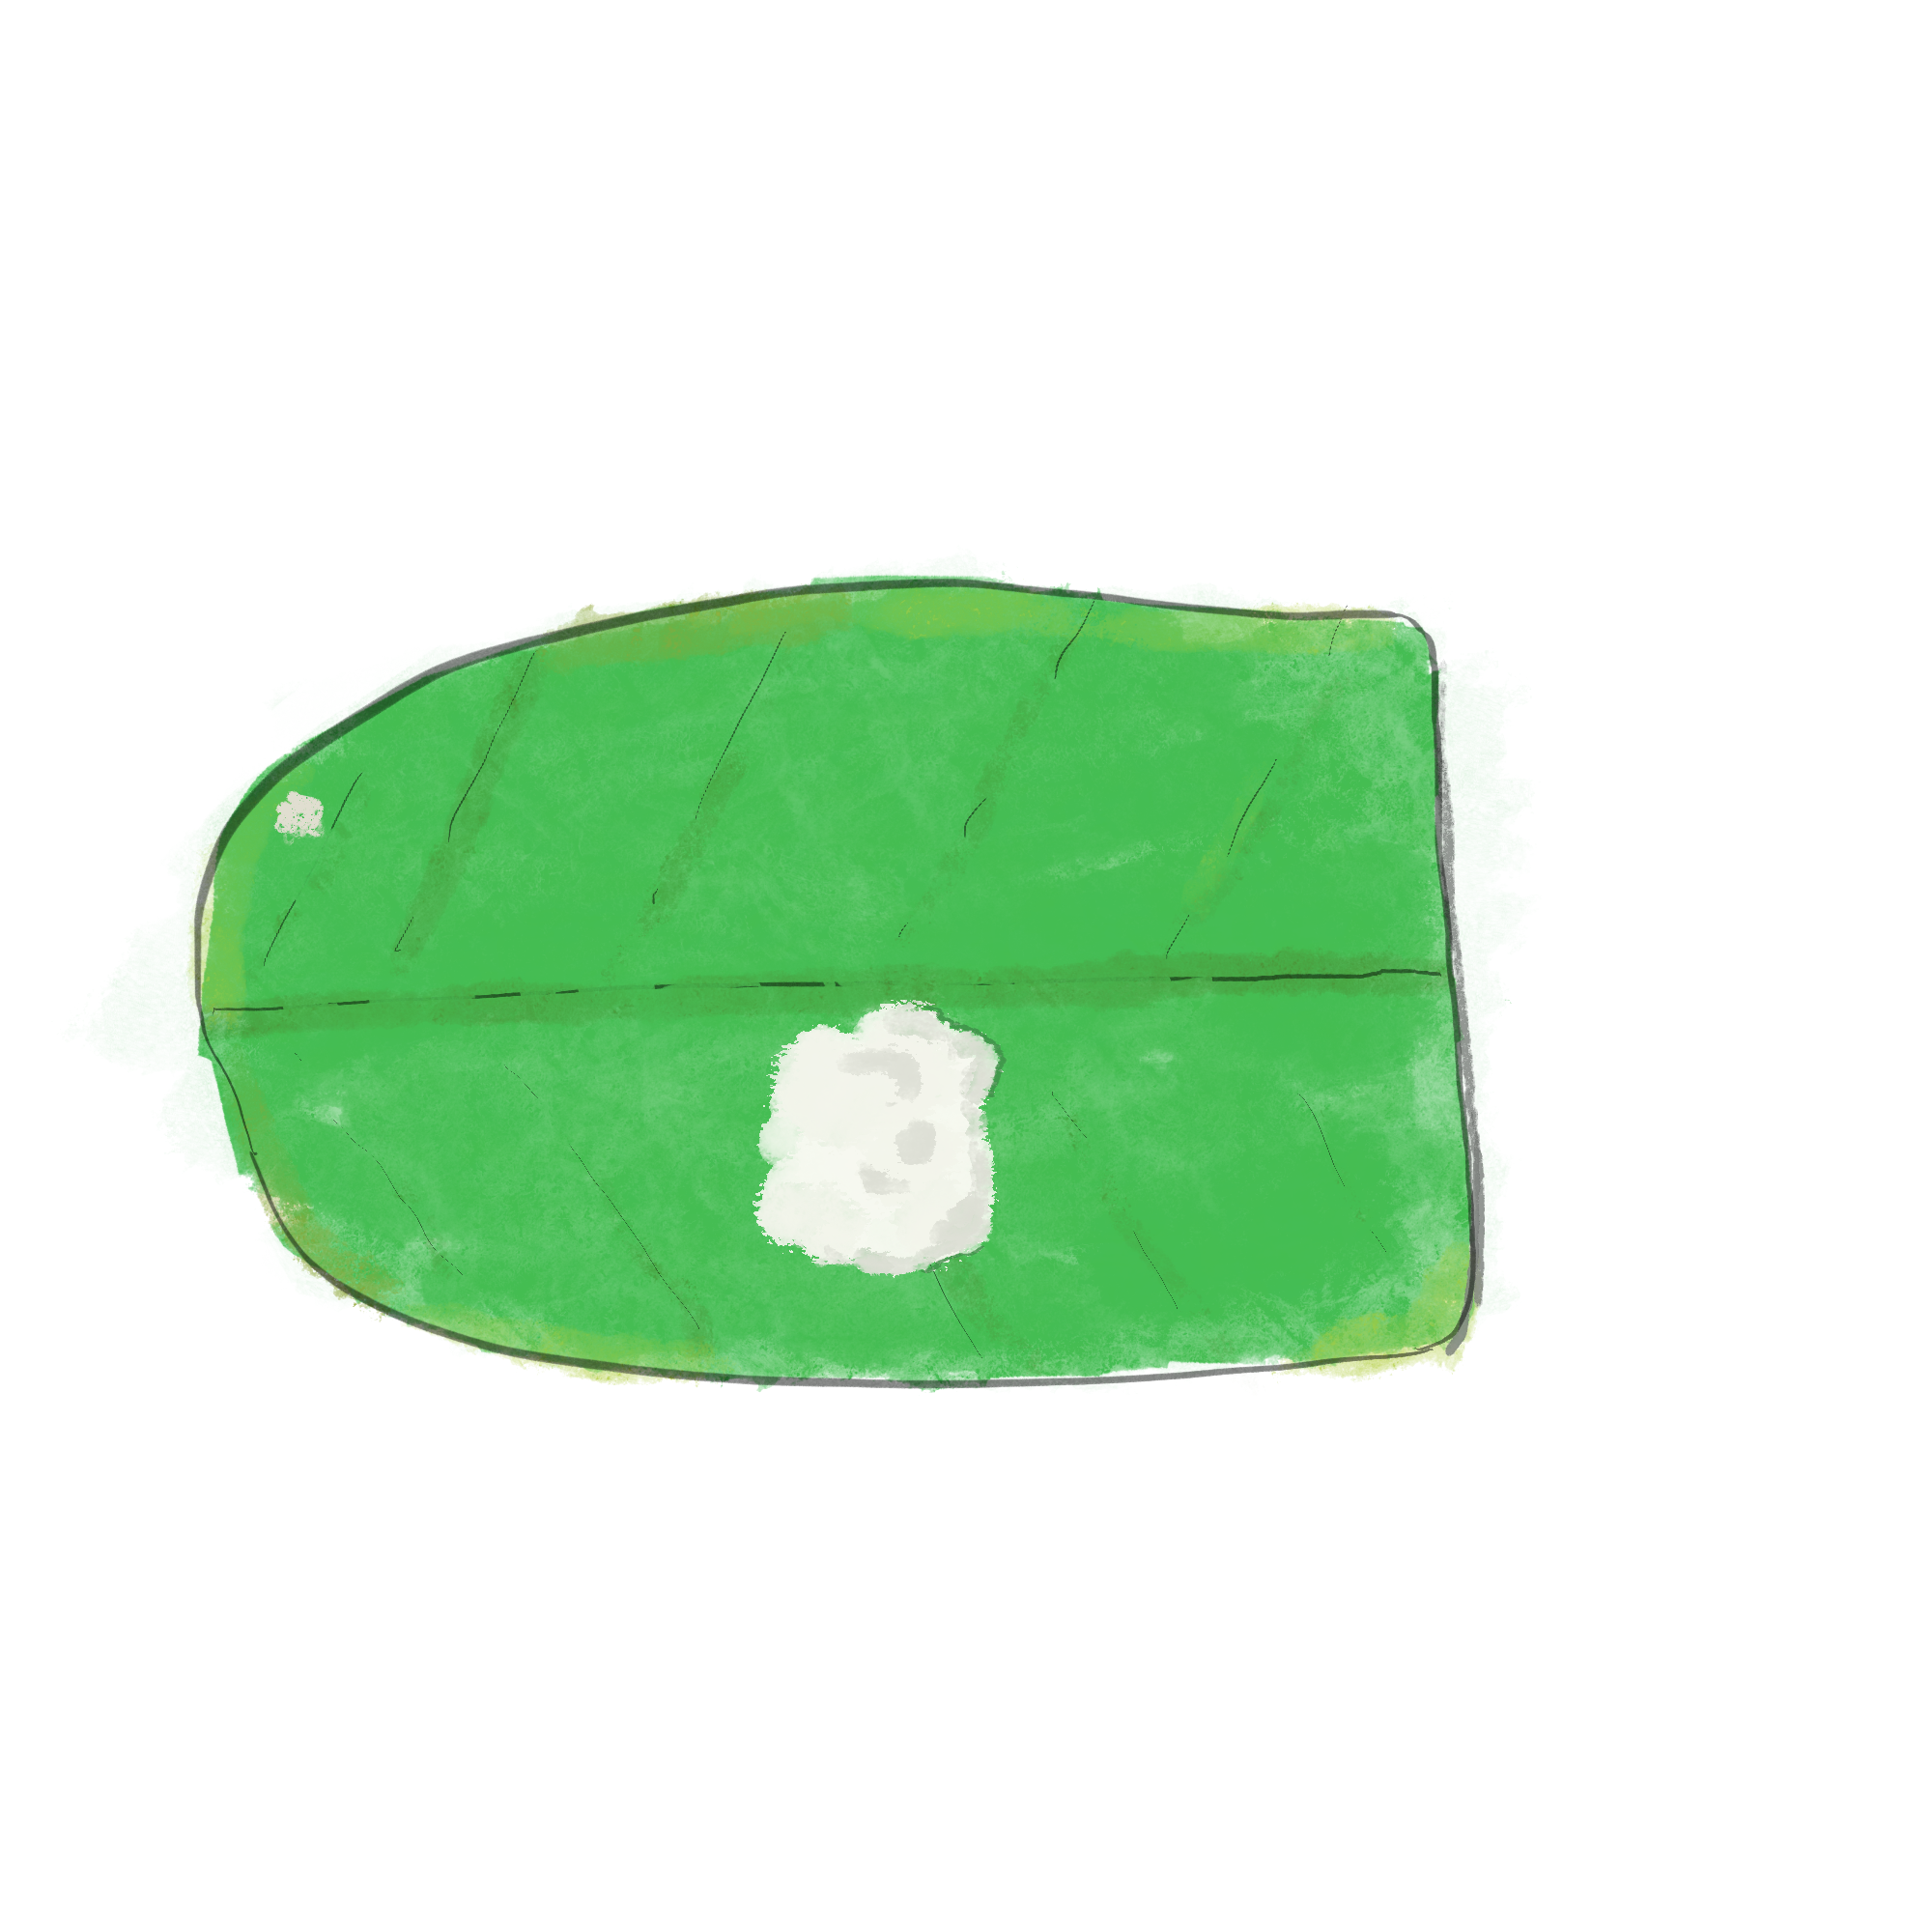
\includegraphics[width=4.0cm]{ele2.png}} % Adjust the coordinates and size as needed
    }
    \AddToShipoutPicture*{
      \put(30,430){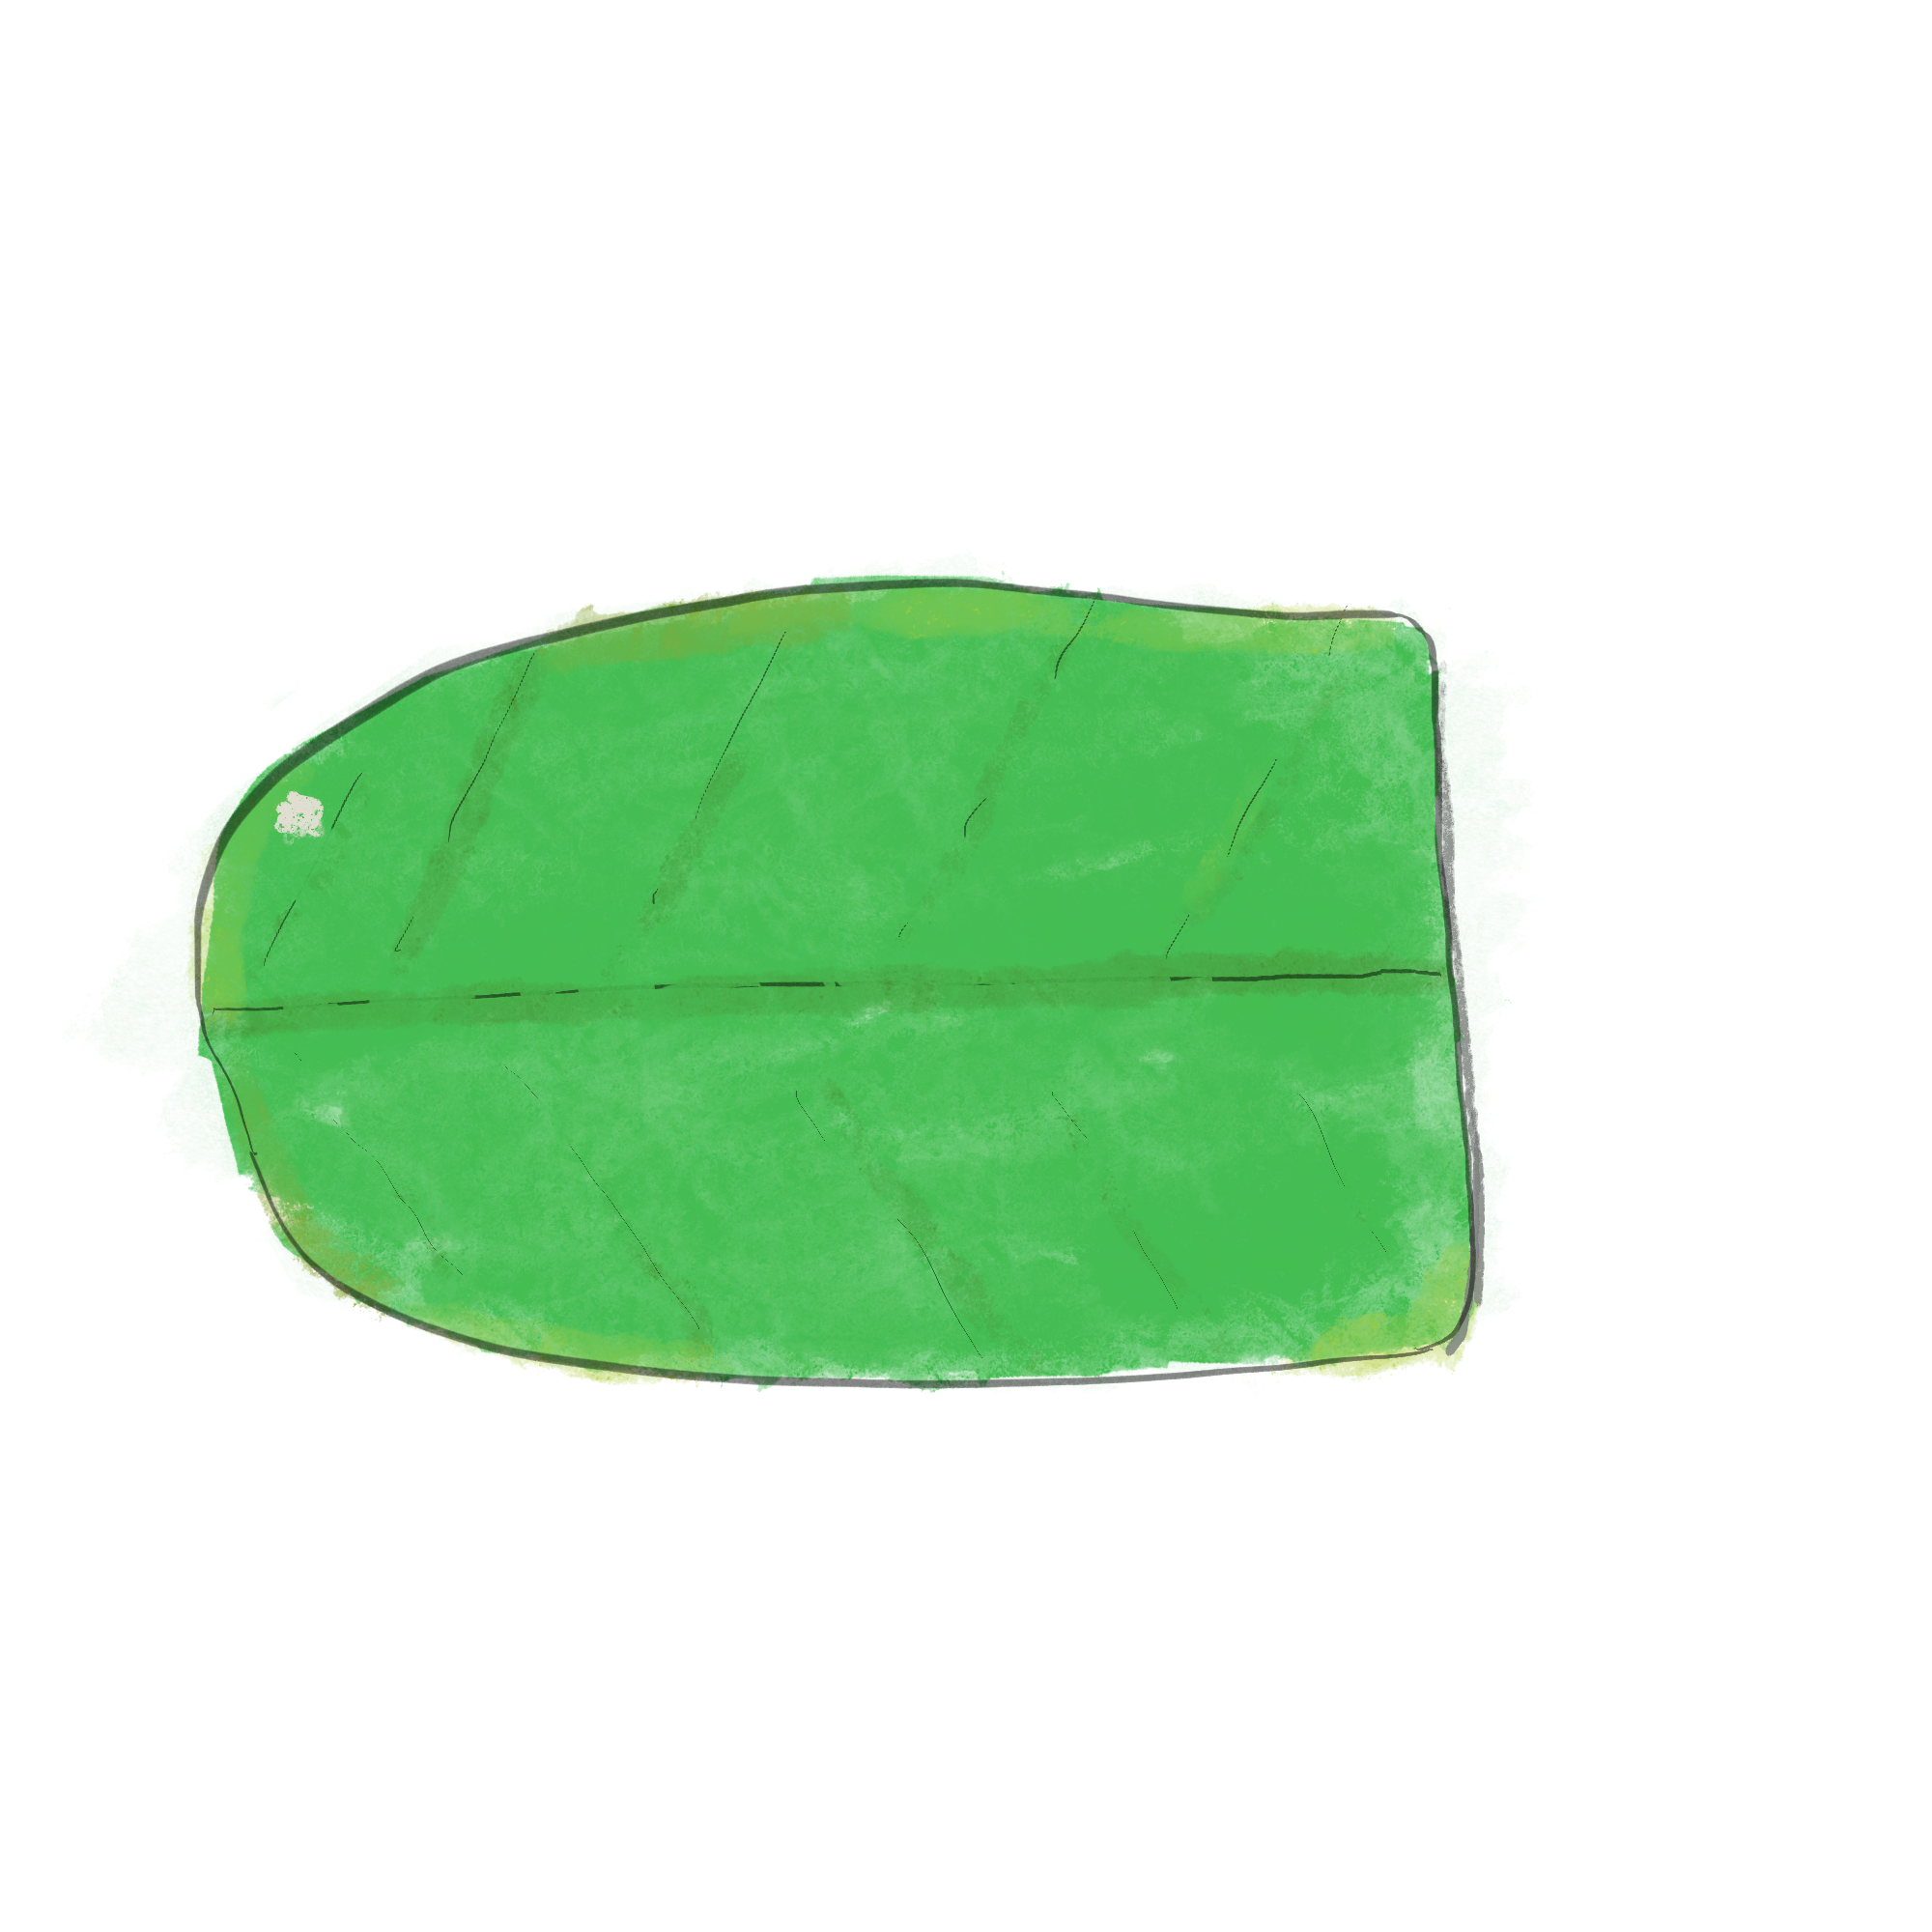
\includegraphics[width=4.0cm]{ele1.png}} % Adjust the coordinates and size as needed
    }
  ಮೂರು ನಾಲ್ಕು ಅನ್ನ ಹಾಕು
  \end{stanza}
  \begin{stanza}
    ಐದು ಆರು ಬೇಳೆ ಸಾರು \verseline
    ಏಳು ಎಂಟು ಪಲ್ಯಕೆ ದಂಟು
  \end{stanza}
  \begin{stanza}
    ಒಂಬತ್ತು ಹತ್ತು ಎಲೆ ಮುದುರೆತ್ತು \verseline
    ಒಂದರಿಂದ ಹತ್ತು ಹೀಗಿತ್ತು
  \end{stanza}
  \begin{stanza}
    ಊಟದ ಆಟವು ಮುಗಿದಿತ್ತು
  \end{stanza}
\end{poem}
\raggedleft
% Add the image as an overlay
%%TODO
}
\end{document}
